\documentclass[a4paper, titlepage, 12pt]{article}

\usepackage{mystyle}
\usepackage[nottoc]{tocbibind}
\usepackage{graphicx}

\graphicspath{ {img/} }

\begin{document}
\begin{titlepage}
\begin{center}
{\large TALLINNA TEHNIKAÜLIKOOL \\
Infotehnoloogia teaduskond \\
Arvutiteaduse instituut}
\vfill
{\large Raigo Aljand} \\
\vspace{7mm}
{\LARGE Assessing Article Quality in Wikipedia Using Machine Learning
Algorithms} \\
\vspace{7mm}
bakalaureusetöö
\vspace{20mm}
\begin{flushright}
Juhendaja:
\begin{minipage}{35mm}
{\large
Jaagup Irve \\
Tarkvarainsener}
\end{minipage}
\end{flushright}
\vfill
Tallinn 2014
\end{center}
\end{titlepage}

\begin{abstract}
[Here you should briefly describe the aims of your work]
[Here you should briefly describe the main problems dealt with]
[Here you should briefly describe the main results obtained]

The thesis is in [language] and contains [pages] pages of text, [chapters]
chapters, [figures] figures, [tables] tables., etc.
\end{abstract}

\listoffigures
\newpage

\listoftables
\tableofcontents
\newpage

\section*{Sissejuhatus}
\addcontentsline{toc}{section}{Sissejuhatus}

\section{Theoretical base}

\subsection{Programming language}
Programming language is a formal language with a set of rules about how the computer should behave. The syntax of the language is usually considered the grammar of the language. For example, if there is a syntax problem in the program, the computer doesn't understand the command and stops. The semantics of the language is considered to be the vocabulary and meaning of the language. If there is a semantical problem, then the program is valid and understandable to the computer, but it is not what the programmer wished to happen. The program will react rather unpredictably. Syntactic sugar is a feature that the programmer can easily implement it in the language and is there for the convenience.

Since a programming language is only a set of rules, it needs an implementation. An implementation is a program that evaluates the syntax into machine actions. There are usually multiple ways to implement this. The most direct approach is to use interpretation, which parses the source code and performs the instructions directly. A second approach is to compile the program, which translates the source code into machine code and optimises it, and then run it. It is also possibe to compile a language into another language and then run from that language's implementation. A compiled program will usually run faster, because the program can be heavily optimised, but compiling the program may take some time. This disadvantage doesn't usually reach the user, because the programmer compiles the program before  publishing the machine code to the user. The user can then choose the right file for its computer architecture. Compiling to a lower language has the advantage that the work of adapting for different processor architectures and optimising is already done, but it is possible to compile to a too general source code, which leads to less optimisations.

A third approach is to use just-in-time (JIT) compilation. JIT takes a hybrid
approach between running it raw and compiling. While running the program, the
JIT compiler will observe what parts of the program are most often run and will
compile those parts. Because the analysation is fairly complex and runs parallel
to the execution of the program, JIT compilers take a lot more
memory.\cite{website:jit-memory} The advantages are that the first operations start
immediately and long programs still run almost as efficiently as a precompiled program. The disadvantages are the high memory usage and sudden pauses in the program execution while the necessary part is being compiled.
Programming languages are usually divided into two categories: high level languages and low level languages. The difference is that low level languages are designed more around how the computer works, while high level languages are designed more around the productivity of the programmer. Because high level languages need to do more translation between what the programmer wants and what the computer accepts, they are usually slower than low level languages. Another advantage of lower level languages is that they enable the programmer to have better access to specific operations and more understanding how the program is executed. This is very useful when the main goal is optimisation.

Another way to divide programming languages is static and dynamic programming languages. A programming language is considered static if it uses static typing. Static typing means that the type of a variable is determined prior to the execution of the program. This way the program doesn't have to check the type of a variable at the time of the execution and, therefore, can run faster. Dynamic typing holds the advantage that a variable can hold different types of values at different times and that types can be changed at runtime.

\subsubsection{Procedural programming}
Imperative programming is a style of programming with the philosophy of changing the machine's state to the required state, which could be a file in a hard drive or a video on the screen. For that the computer executes a sequence of operations in order, which are specified by the programmer. An operation is some change of state in the computer or calculation of some data.

Procedural programming is a subset of imperative programming. Procedural programming tries to divide the program into variables, data structures and procedures. Procedures are meant to group together abstract operations so they could be reused in different situations. In this case an operation can also be a procedure. Data structures are meant to group together conjoined data so they could be moved and manipulated more easily. Variables are pointers to data. They point to the location of the data in the memory which can be then easily retrieved.

\subsubsection{Object-oriented programming}
Object-oriented programming is another subset of imperative programming. Object-oriented programming tries to divide the program into objects that communicate with each other. Each object has fields and methods. Fields and methods are similar to variables and procedures, but they are tied to the object. Fields are considered to be the objects inner state and methods are considered to be the object's behaviour or object's interface.

The goal of object-oriented programming is encapsulation. Encapsulation means
that each object has an inner state, inner behaviour and an interface for other
objects to use. An outer object doesn't need to know what is happening within
the object. It only needs to know how the object is going to react to an
interface procedure. Access protection modifiers are generally employed to
better enforce this behaviour. These modifiers are usually tied to a method or
field and they describe what other methods are allowed to access these methods
or fields. Right to access a field means the right to read or change the field
and right to access a method means the right to run the
method.\cite{access-modifiers}
An object's methods always have access to its objects fields.

An object can inherit another object. The inheriting object is called subobject and the inherited object is called the superobject. The subobject gets the superobject's fields and methods. A copy of the superobject is created and retained in the subobject. When searching for the subobject's methods or fields and they are not found then the superobject is searched for the field or method. A subobject doesn't automatically have access to the superobject's private fields and methods. The subobject can override the superobject's public methods. The type signature of the method cannot change, but the content or the action of the method is changed.

\emph{The classic way to implement object-oriented programming is with classes.} In class-based programming the object is separated into the class and the instance. The class is an abstraction and the classification of the object while the instance is a actual object with actual data. Usually the class holds the behaviour of the object, which includes the constructor. The constructor is a special method, that is called when a new instance is being created from the object. Inheritance works by remembering the inheritance line and then searching for the methods in the right class.

An interface is a a class that has no fields and all its methods are public. All of the methods are abstract methods, meaning that the methods have no content or implementation. A class can usually implement multiple interfaces but inherit from only one class. One can't make a instance of an interface, there needs to be an implementing class. An abstract class is a class that has atleast one abstract method. Similar to interfaces, it is impossible to make an instance of them. However they are still classes and and they are inherited, not implemented.

\emph{In my humble opinion the rawest object-oriented programming style is protoype-based programming.} Prototype-based programming is more used by dynamic languages. It keeps the design of the language minimal by having no wrappers around objects and their attributes. An object is created by creating an empty object or by cloning an existing object. Inheritance works by cloning an existing object and the subtype can replace the old attributes or add new attributes. Abstract objects are objects that will hold only behviour by containing only constant or default attributes.

\subsubsection{Functional programming}
Functional programming languages are designed around functions. Programming functions are similar to mathematical functions, that it has inputs as parameters and returns a value as output. A function should always return the same output with the same inputs and the inputs should not be changed inside the function. This leads to a particularly stateless form of programming.

Due to the stateless form of this style, functional programming languages usually support immutable datastuctures. Instead of updating a datastructure, it is copied with the new values replaced and the new datastucture is returned. First-class functions and dynamic evaluation of functions are also supported.


\subsection{Client-server architecture}
Client is process that requires some service. Server offers that service. The client and server communicate with HTTP. HTTP is a protocol in which the client sends the server a request and the server processes the request and sends a response. HTTP is purely plaintext. The HTTP request is divided into headers and content. The request has an URL in the header. URL stands for Uniform Resource Locator. It is a way for the client to request a certain page or other resource on the server. Another thing that the URL can contain are extra parameters. From those parameters the server can return the resource in a different form. Usually the request content is empty.

Extensible Markup Language (XML) is a protocol to describe data. It tries to nest data between descriptive tags. The tags can be nested and the tags can have attributes. The tags are not preset, so every user can design it's own way of presenting data. The syntax of a XML tag is \texttt{<tag attribute1=“value1“ attribute2=“value2“>data</tag>}. A tag can't have the same attribute with different values. data can be normal text or more tags. \texttt{<tag />} is shorthand for \texttt{<tag></tag>} for when the user doesn't have data to insert.

The HTTP response also splits into a header and content. Inside the content is usually the requested data. A browser is an application that sends HTTP requests to servers and parses and visualises the response to the user. To help with the visualisation and interactiveness of the pages, HTML was created. HTML is an Extensible Markup Language (XML) where the tags are focused on giving text some form of context. For example, the a is a tag for a link and the \texttt{h1} is a tag for a level 1 header. The browser also parses the HTML into visual cues and interactions with the user.

Often the tags in HTML aren't enough. For that there is JavaScript (JS). JavaScript is a dynamic general-purpose programming language. JavaScript works by registering a JavaScript function with an HTML event, so that when that event is fired, that JavaScript function is run. JavaScript interacts with the user by changing the current HTML the user is seeing. Because JavaScript is a general-purpose programming language, unlike HTML, any arbitrary calculation is possible. JavaScript uses Asynchronous JavaScript and XML (AJAX) to send HTTP requests to outside servers. Despite the name, the returned format doesn't have to be XML.

HTML pages are purely intended for browsers to parse and a human to see. For an
another application to get data from a HTML page, it has to web scrape. Web
scraping is observing beforehand how a web page is built and later filtering out
the necessary data from the HTML. Another way is for the server to offer an
Application Programming Interface (API). An API is a way for a program to get
data from the server with a HTTP requst in a more formal and machine-friendly
form. There are multiple formats for getting the data: JavaSrict Object Notation
(JSON), a Domain specific XML and so on.

With JSON the HTTP content is one legal JavaScript Object, which makes it easy
to read into JavaScript. Another advantage of it over XML is that there is basic
type checking. Javascript allows a value to have a few different types with
different notations: a string, a number, another object, an array; and the three
constant values \verb;true;, \verb;false;,
\verb;null;.\cite{website:json-guide,website:json}


\subsection{Machine learning}
Machine learning is used when the programmer doesn't know all about the domain he is writing for. It is then necessary to have the machine learn by itself by some criteria. Machine learning generally divides into two categories: supervised learning and unsupervised learning. Supervised learning is when you have a known data set where for a known input there will be a known output. In unsupervised learning there is no such data set and the programmer is mostly looking for correlation between the inputs. Unsupervised learning is mostly used for data mining.

Logistic regression is a form of supervised learning which is used for classification. Our dataset $D$ will consist of the input of the model, a matrix of the the vectors $\mathbf{x_n}$ and the required outputs $y_n$ for the inputs. A input vector $\mathbf{x_n}$ will consist of the numerical features of the data prefixed with a 1 for the bias. $y_n$ can have only 2 values: 1 or -1. There are more complex forms of logistic regression that can handle more than two values for $y$ but is out of the scope of this paper. $N$ will be the size of our dataset.
\[ D = \{ (\mathbf{x_1}, y_1), (\mathbf{x_2}, y_2), \ldots, (\mathbf{x_N}, y_N)\} \]
\[ \mathbf{x_n} = [ \begin{array}{cccc} 1 & x_1 & \ldots & x_d\end{array} ]^T \]
Similar to another supervised learning algorithm linear regression, logistic
regression is a linear model.``All linear models make use of a "signal" $s$
which is a linear combination of the input vector $\mathbf{x}$ components
weighed by the corresponding components in a weight vector
$\mathbf{w}$.''\cite{logistic-regression}
\[\mathbf{w} = \left[\begin{array}{cccc} w_0 & w_1 & \ldots & w_d \end{array}
\right]^T \] \[s = w_0 + w_1 x_1 + \cdots + w_d x_d = \sum_{i=0}^d w_i x_i =
\mathbf{w} \cdot \mathbf{x} = \mathbf{w}^T \mathbf{x}\] Linear regression will use the signal directly as output, but logistic regression will pass the signal through a sigmoid or logistic function and treat thats output as the probability that $y=1$.
\[h(\mathbf{x}) = \theta(s)\]
\[\theta(s) = \frac{e^s}{1+e^s} = \frac{1}{1 + e^{-s}}\]

%\usepackage{graphics} is needed for \includegraphics
\begin{figure}[htp]
\begin{center}
  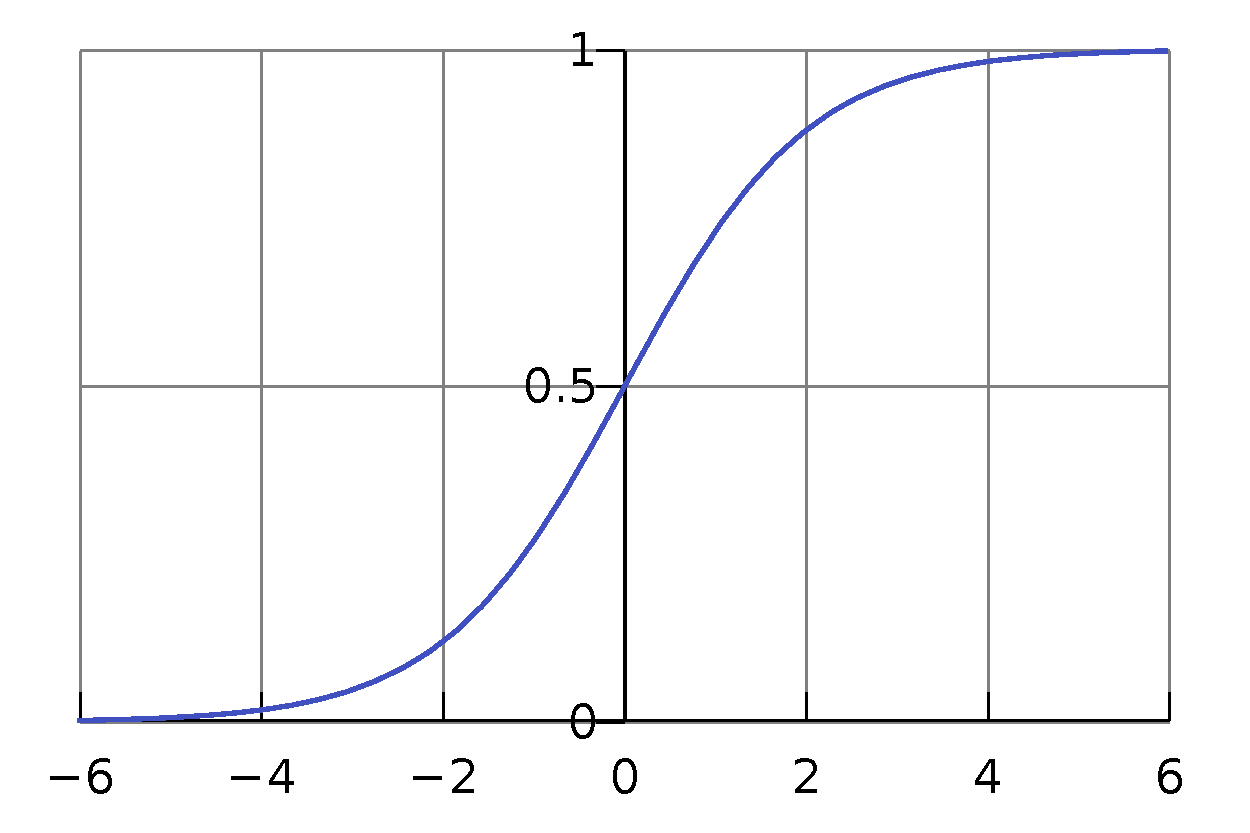
\includegraphics[width=\textwidth]{logistics-curve}
  \caption[Logistics curve]{The shape of a logistics curve.}
  \label{logistics-curve}
\end{center}
\end{figure}

As shown in figure \ref{logistics-curve}, the logistic function is good for
translating between linear values and probability, because the higher the linear value, the higher the probability of the output value being 1 and the lower the linear value the higher the probability of the output being -1. At input value 0, the probability of it being either value is 0.5.

``We say that the data is generated by a noisy
target.''\cite{logistic-regression} 
\[ P(y|\mathbf{x}) = \left\{
\begin{array}{ll}
f(\mathbf{x}) & \mbox{for } y = +1 \\
1 - f(\mathbf{x}) & \mbox{for } y = -1
\end{array} \right. \]
We want to learn a hypothesis $h(x)$ that best fits the above target according to some error function.
\[h(\mathbf{x}) = \theta \left( \mathbf{w}^T \mathbf{x} \right)\approx f(\mathbf{x})\]
``It's important to note that the data does not tell you the probability of a
label but rather what label the sample has after being generated by the target
distribution.''\cite{logistic-regression}. The goal of the training will be to calculate the weight vector w so that it minimizes some kind of in-sample error measure.
\[\mathbf{w}_h = \argmin_w E_{in} (\mathbf{w})\]
Our error measure will be based on likelihood. Likelihood is the probability of generating the data with a model. Likelihood will be high if the hypothesis is similar to the target distribution. \emph{TODO: Controversy? What? Millegipärast pidi likelihood olema controversial, aga ma ei saanud aru, miks.} Let's assume that the data was generated by the hypothesis:
\[P(y|\mathbf{x}) = \left\{ 
\begin{array}{ll}
h(\mathbf{x}) & \mbox{for } y = + 1 \\
1 - h(\mathbf{x}) & \mbox{for } y = -1
\end{array}
\right.\]
\[h(\mathbf{x}) = \theta (\mathbf{w}^T \mathbf{x})\]
Let's try to remove the cases using the property $\theta(-s) = 1 - \theta (s)$.
\[\left.
\begin{array}{l}
\mbox{if $y=+1$ then } h(\mathbf{x}) = \theta (\mathbf{w}^T \mathbf{x}) = \theta (y \mathbf{w}^T \mathbf{x}) \\
\mbox{if $y=-1$ then } 1 - h(\mathbf{x}) = 1 - \theta (\mathbf{w}^T \mathbf{x}) = \theta (-\mathbf{w}^T \mathbf{x}) = \theta (y \mathbf{w}^T \mathbf{x})
\end{array}
\right\} P(y | \mathbf{x}) = \theta(y \mathbf{w}^T \mathbf{x})\]
Let's denote an arbitrary hypothesis g, in which case the likelyhood is defined as:
\[L(D|g) = \prod_{n=1}^N P(y_n | \mathbf{x}_n) = \prod_{n=1}^N \theta(y_n \mathbf{w}_g^T \mathbf{x}_n)\]
To find the best hypothesis, we have to find the best weight vector $\mathbf{w}$.
\begin{eqnarray*}
\mathbf{w} & = & \argmax_\mathbf{w} L \left( D|h \right) = \argmax_\mathbf{w} \prod_{n=1}^N  \theta \left( y_n \mathbf{w}^T \mathbf{x}_n \right) = \argmax_\mathbf{w} \ln \left( \prod_{n=1}^N \theta\left( y_n \mathbf{w}^T \mathbf{x}_n \right) \right) \\
& = & \argmax_\mathbf{w} \frac{1}{N} \ln \left( \prod_{n=1}^N \theta \left( y_n \mathbf{w}^T \mathbf{x}_n \right) \right) = \argmin_\mathbf{w} \left[ - \frac{1}{N} \ln \left( \prod_{n=1}^N \theta \left( y_n \mathbf{w}^T \mathbf{x} \right) \right) \right] \\
& = & \argmin_\mathbf{w} \frac{1}{N} \sum_{n=1}^N \ln \left( \frac{1}{\theta \left( y_n \mathbf{w}^T \mathbf{x}_n \right)} \right) = \argmin_\mathbf{w} \frac{1}{N} \sum_{n=1}^N \ln \left( 1 + e^{-y_n \mathbf{w}^T \mathbf{x}_n} \right)
\end{eqnarray*}
We have derived a good form for the error measure, which is the loss function or the average point error.
\[ E_{in} \left( \mathbf{w} \right) = \frac{1}{N} \sum_{n=1}^N \ln \left( 1 + e^{-y_n \mathbf{x}_n \mathbf{w}^T} \right) = \frac{1}{N} \sum_{n=1}^N e \left( h \left( \mathbf{x}_n \right), y_n \right) \]
\[ e \left( h \left( \mathbf{x}_n \right), y_n \right) = \ln \left( 1 + e^{-y_n \mathbf{x}_n \mathbf{w}^T} \right) \]
We minimise the error function using gradient descent. Gradient descent works by moving the current value towards the local minimum. With the derivative, one can calculate the necessary direction and the rough distance of the local minimum from the current value. Therefore training works with the formula:
\[ \mathbf{w}_{i+1} = \mathbf{w}_i - \eta \nabla E_{in} \left( \mathbf{w}_i \right) \]
Where $\eta$ is the learning rate. We need the derivative of the point error function and the average point error.
\[ \frac{d}{d \mathbf{w}} e \left( h \left( \mathbf{x}_n \right), y_n \right) = \frac{-y_n \mathbf{x}_n e^{-y_n \mathbf{w}^T \mathbf{x}_n}}{1 + e^{-y_n \mathbf{w}^T \mathbf{x}_n}} = -\frac{y_n \mathbf{x}_n}{1 + e^{y_n \mathbf{w}^T \mathbf{x}_n}} \]
\begin{eqnarray*}
\nabla E_{in} \left( \mathbf{w} \right) & = & \frac{d}{d \mathbf{w}} \left[ \frac{1}{N} \sum_{n=1}^N e \left( h \left( \mathbf{x}_n \right), y_n \right) \right] = \frac{1}{N} \sum_{n=1}^N \frac{d}{d \mathbf{w}} e \left( h \left( \mathbf{x}_n \right), y_n \right) \\
& = & \frac{1}{N} \sum_{n=1}^N \left( -\frac{y_n \mathbf{x}_n}{1 + e^{y_n \mathbf{w}^T \mathbf{x}_n}} \right) = - \frac{1}{N} \sum_{n=1}^N \frac{y_n \mathbf{x}_n}{1 + e^{y_n \mathbf{w}^T \mathbf{x}_n}}
\end{eqnarray*}
\[ \mathbf{w}_{i+1} = \mathbf{w}_i - \eta \left( -\frac{1}{N} \sum_{n=1}^N \frac{y_n \mathbf{x}_n}{1 + e^{y_n \mathbf{w}_i^T \mathbf{x}_n}} \right) = \mathbf{w}_i + \eta \left( \frac{1}{N} \sum_{n=1}^N \frac{y_n \mathbf{x}_n}{1 + e^{y_n \mathbf{w}_i^T \mathbf{x}_n}} \right) \]
To lower the number of iterations, each feature of $\mathbf{x}$ should be normalised before it is used for predicting or training the model. Normalising means that the program calculates the standard score of each of the features which is then used instead. The standard score subtracts the mean from the features and divides that with the standard deviation of the values. A values standard score floats around the 0 value and roughly has the same absolute value as other standard scores. When normalising $\mathbf{x}$ for predicting, the mean and standard deviation cannot be enhanced with that data, because then the trained model will not be expecting such data. It would mean comparing two fundamentally different sets of data. It is important to note that the bias variable in $\mathbf{x}$ should not be normalised, because it will end in a divide by zero error.


\section{Used technologies}
\subsection{Python}
In this project I used Python version 2.7.

Python is a widely-used, general-purpose programming language as shown in figure
\ref{python-popularity}. Python focuses on human readability, simplicity and
power to the
programmer.\cite{website:python-zen,website:python-faq-creation-reason} That
fact is most likely best expressed by the fact that Python uses indentation to
divide its blocks. A language like C uses the curly braces for that and uses the
indentation only for clarity of reading. Python, however, forces the programmer
to make the program more readable and standardised. Semantically Python is very
flexible. It supports functional, object-oriented and procedural programming
styles.

% \usepackage{graphics} is needed for \includegraphics
\begin{figure}[htp]
\begin{center}
  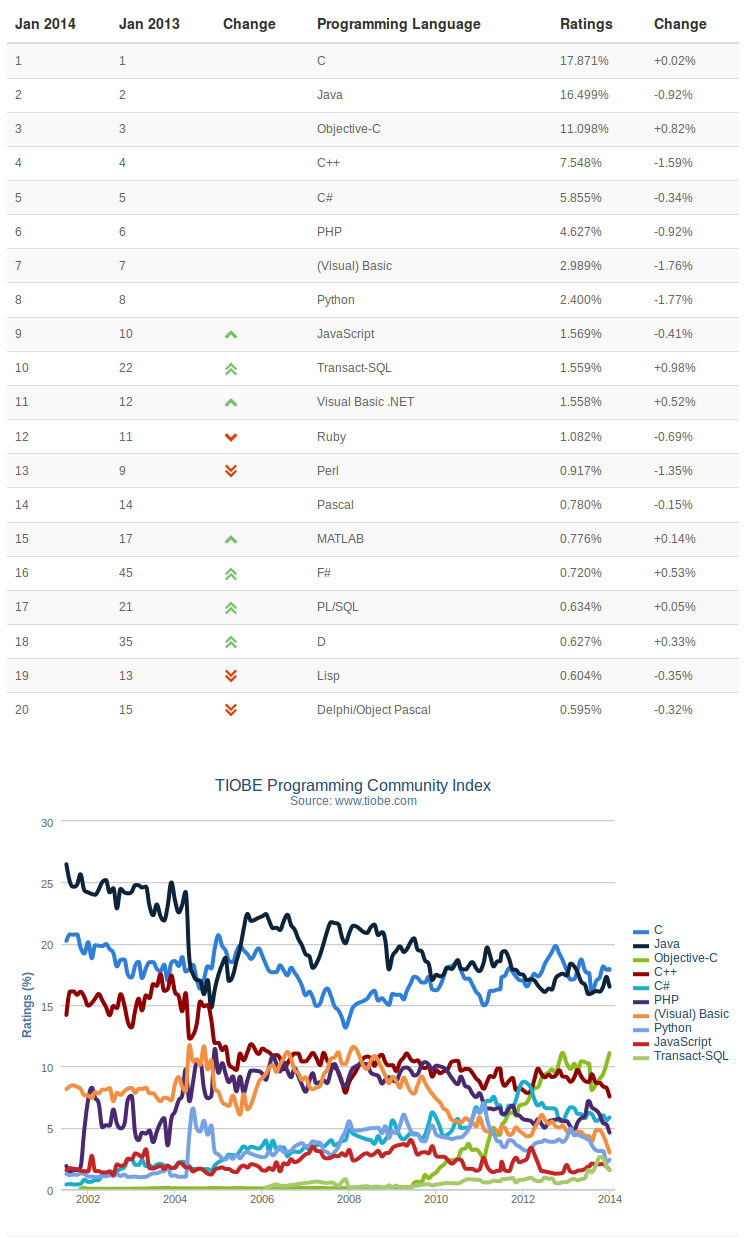
\includegraphics[height=564pt]{tiobe}
  \caption[Python popularity]{Popularity of python compared to other
  languages\cite{website:tiobe-index}}
  \label{python-popularity}
\end{center}
\end{figure}

To minimise clutter in the language, Python uses dynamic typing, also called
duck typing. Duck typing doesn't check if an object implements some certain
interface, but simply tries to call or use the method or attribute. The
principle is ``If it looks like a duck and quacks like a duck, it must be a
duck''.\cite[duck-typing]{website:python-glossary} This makes it possible to not use
interfaces and generics in the code.

Python has two running modes: the interactive mode and the script mode. The
interactive mode is a read-eval-print loop. It reads the user supplied
expression and parses it into a data structure, evaluates it and prints the
result. An expression can't be multiline and must return only one value.
Evaluating a value will return that value and evaluating a variable returns the
contents of the variable. The script running mode is similar to the interactive
mode, but instead of the user, the expressions are taken from a file and when
the end of the file is reached, the interpreter terminates.

\subsubsection{Procedural style}
Each file in python is a module with the same name as the filename, except without the \texttt{.py} extension. Each module can import another module or every object in another modules namespace with the \texttt{import} command. When the import command is evaluated, the whole file is evaluated once. A directory can also be a module if it contains a \texttt{\_\_init\_\_.py} file. In that case the module is initialised with the \texttt{\_\_init\_\_.py} file and it's namespace contains the file modules in the directory.

Procedures in Python are called functions, because they can return one or multiple values, however if a return value isn't specified, it returns the \texttt{None} value. Python uses pass by reference so that values inside the object can be changed. However one must still be careful that changing the reference itself won't change the reference in the caller. Also even though numbers are objects and therefore are passed by reference, they are immutable and one can't change their inner value. That makes them in essence pass by value.

The closest feature that gets to a C style stucture is the named tuple. A named tuple is a factory function that will create and return a class. A tuple is an immutable list. The inputs of the function are the class name, the fields of the class and more optional parameters. The returned class inherits from the tuple type and only accepts the previously entered fields. An example:

\begin{verbatim}
>>> Point = namedtuple('Point', ['x', 'y'], verbose=True)
class Point(tuple):
    'Point(x, y)'

    __slots__ = ()

    _fields = ('x', 'y')

    def __new__(_cls, x, y):
        'Create a new instance of Point(x, y)'
        return _tuple.__new__(_cls, (x, y))

    @classmethod
    def _make(cls, iterable, new=tuple.__new__, len=len):
        'Make a new Point object from a sequence or iterable'
        result = new(cls, iterable)
        if len(result) != 2:
            raise TypeError('Expected 2 arguments, got %d' % len(result))
        return result

    def __repr__(self):
        'Return a nicely formatted representation string'
        return 'Point(x=%r, y=%r)' % self

    def _asdict(self):
        'Return a new OrderedDict which maps field names to their values'
        return OrderedDict(zip(self._fields, self))

    def _replace(_self, **kwds):
        'Return a new Point object replacing specified fields with new values'
        result = _self._make(map(kwds.pop, ('x', 'y'), _self))
        if kwds:
            raise ValueError('Got unexpected field names: %r' % kwds.keys())
        return result

    def __getnewargs__(self):
        'Return self as a plain tuple.   Used by copy and pickle.'
        return tuple(self)

    __dict__ = _property(_asdict)

    def __getstate__(self):
        'Exclude the OrderedDict from pickling'
        pass

    x = _property(_itemgetter(0), doc='Alias for field number 0')

    y = _property(_itemgetter(1), doc='Alias for field number 1')


>>> p = Point(11, y=22)     # instantiate with positional or keyword arguments
>>> p[0] + p[1]             # indexable like the plain tuple (11, 22)
33
>>> x, y = p                # unpack like a regular tuple
>>> x, y
(11, 22)
>>> p.x + p.y               # fields also accessible by name
33
>>> p                       # readable __repr__ with a name=value style
Point(x=11, y=22)
\end{verbatim}

If a variable is nonlocal and the variable in the function is only read, then the interpreter will try to find it from a nonlocal context. However, if the variable is given new value anywhere in the function, the interpreter will assume that the variable is local and the global variable will not be visible. One can make a variable global with the \texttt{global} command. The syntax is \texttt{global variable}. After that, every reference to the variable will be a reference to the global variable.

\subsubsection{Functional style}

% TODO This is wrong: first explain def and then say lambda as the limited form
% of def. I don't really care right now, though.
Python has full support for first-class functions meaning that a function is an
object like any other value. One defines a function with the \texttt{lambda}
keyword or with the \texttt{def} keyword. \texttt{lambda} and \texttt{def} are
very similar, but \texttt{def} binds the function value to an identifier and
\texttt{def} implicitly returns \texttt{None}. For \texttt{def} to return
anything, it needs the \texttt{return} keyword. \texttt{lambda} is more
constrained. It is not allowed to be multiline and it is only allowed to have
one expression. The expressions value is then implicitly returned. The syntax of
\verb;def; and \verb;lambda; are:
\begin{verbatim}
def fib(n):
    a, b = 0, 1
    while a < n:
        print a,
        a, b = b, a+b
    return a

f = lambda x: x**2

# Now call the function we just defined:
f(2000)
fib(2000)
\end{verbatim}
After the \verb;def; command comes the name of the function, then inside the
brackets are the names of the parameters of the function separated by a colon.
A function can have optional parameters by giving the parameter a default value
like this: \verb;parameter=value;. The expression of the value is only
evaluated once, so if the parameters value is changed during the call of the
evaluation of the function, the change will be seen in the future evaluations
of the function. On the next lines is the body of the function.

The \verb;lambda; command doesn't take a name, therefore brackets are not
necessary and the parameters simply follow the \verb;lambda; command again
separated by commas. After the colon is the expression to be returned. After
the definition and binding to an identity, both function values are of the same
type and follow the same rules.

Python also has lexical closures, which gives the function a strong reference to
the namespace. This excludes the possibility that the namespace will be garbage
collected while the function is still in memory. The function has the guarantee
that the non-local values will exist even after the enclosing context is deleted
or garbage collected.\cite{website:python-closures}

Generator is a data structure to dynamically iterate items. When a function has
a \texttt{yield} command somewhere inside of the function, when the function is
evaluated, the function is actually not run, but a generator data structure is
returned. The \texttt{yield} command is very similar to \texttt{return}, except
for one difference. When the generator is iterated, for example in a
\texttt{for} loop, the function is run until a \texttt{yield} command is hit,
the value is returned and the function is paused. When the next element is
requested, the function is continued again until the next \texttt{yield}. This
continues until the function reached the end, which signals that the generator
has no more elements.
\begin{verbatim}
def generate_ints(N):
    for i in range(N):
        yield i
\end{verbatim}
The advantage of a generator over a list for example, is that lists require that
all their elements are in memory at some point, while a generator has only one
element at a time in memory. Because when using a generator one can iterate over the items only once, there is also a slight speed increase. The disadvantages are that generators have no such data as the length of the iteration, are immutable and can't be iterated over for a second time.

Since other functional languages have them, Python also has functions
\verb;map;, \verb;filter; and \verb;reduce;. \verb;map; applies a function
to every item in an iterable and returns a new list with the results of the
function. \verb;filter; applies a function to every item in an iterable and
returns a new list with the items where the function returned \verb;True;. And \verb;reduce; applies a function for every item in an iterable and returns the value of the last evaluation. In this case the function must have two parameters and the first parameter holds the value from the last evaluation of the function.

A way to avoid using \verb;map; and \verb;filter; is by generator expressions
and list comprehensions. List comprehensions are a syntactic sugar to easily
create lists. Unlike \verb;map;, list comprehensions don't need to be supplied a
function, but can also use arbitrary expressions. A sample list comprehension
is: \verb;[2 * item for item in iterable if item % 2 == 0];. This expression
returns a filtered list where each element of iterable is multiplied with 2. The returned list contains only elements that were even before. Therefore the syntax is \texttt{[expression for expr1 in sequence1 if condition1 for expr2 in sequence2 if condition2 ...]}. The commands are nested with the right being inside the left and the first expression being the returned innermost expression. Generator expressions are syntactically same, except normal brackets instead of square brackets are used and they create a generator instead of a list.

\subsubsection{Object-oriented style}
Python has a class-based object-oriented style. Python, however, is more dynamic than a normal static class-based language like Java. After an object has been created from a class, one can still change that concrete object's variables and methods. Every property is also public. Properties, that the programmer considers private, are usually prefixed with underscores. Each statement is evaluated top to bottom. If there are multiple properties with the same name, then the last evaluated property is remembered.
\begin{verbatim}
class MyClass:
    """A simple example class"""
    i = 12345
    def f(self):
        return 'hello world'
\end{verbatim}
In Python, methods are functions, that get the object's instance in the first parameter, but are called with the first parameter ignored, like this: \verb;my_object.f();. If there are brackets after the class name and another class's name inside the brackets, the class inherits from the class in the bracket. A method can access the superclass with the \verb;super; function. The super function takes two arguments: the type of the class of whose the super is being searched for and the second is the object.

Multiple inheritance is supported by putting multiple class names in the brackets supported by comas. If called for a property, that a object doesn't have, the environment will try to find the property from the first named superclass recursively until it hits object class and then the next superclass recursively and so on. The object class is the superclass of every class. If there are no brackets or the brackets are empty, then the object class is an implicit superclass.

\subsubsection{Implementation}

The official implementation of Python is CPython. Every formal change to the
language will be almost immediately mirrored in this implementation. It will be
supported for a long time will be the most current and up-to-date compared to
other implementations. CPython is a bytecode interpreter. It compiles to an
intermediate bytecode, which it then interprets. It compiles every time the
source file has been changed. This implementation is slow compared to
other languages\cite{website:python-speed}, but enables hooking the script to a
C module. Since the C programming language is fast,\cite{website:c-vs-python} it
is possible to write most of the program in Python and write the bottlenecks in
C.

{
\newcommand{\pypy}{PyPy}

The most popular alternative implementation to CPython is \pypy. \pypy{} is a JIT
compiler written in Python. It is popular because of its speed. As of \today,
\pypy{} is about 6.2~times faster than pure
CPython.\cite{website:python-pypy-speed} There are two disadvantages: \pypy{}
doesn't have hooks into C and PyPy isn't as up-to-date as CPython. As of \today,
Python 3 support for \pypy is in the beta state while CPython supports Python
3.4.0. Also since PyPy doesn't have hooks into C, it can't speed up the
bottlenecks of a program. With simple calculation from
\cite{website:c-vs-python,website:python-pypy-speed}, C gcc is still about 3
times faster than PyPy.
}


There are also Jython and IronPython. Jython compiles down to Java bytecode. It
allows the programmer to use libraries from Java in his project. IronPython is
the same principle, only it compiles to the .NET bytecode. That gives IronPython
projects access to .NET libraries.


\subsection{MediaWiki}
A wiki page is a page that owns a title in that wiki and is supposed to
aggregate information on the world wide web about the subject of the title. Most
of the content in the wiki pages are created or changed by the users of the
wiki. MediaWiki is software for a content-classification wiki. A content
classification wiki forbids writing personal knowledge and opinions on the wiki
page and only allows writing information that can be referenced. MediaWiki has a
separarate web page for discussion.\cite{wiki:mediawiki-about}

An interwiki link is a link that refers to another wiki page in the same wiki.
This way wikis don't have to duplicate information on different pages and just
refer to an another page. Links that link to outside the wiki are called
external links. Usually external links are in the page as references. There are
a special type of wiki pages that are called templates. They are not meant to
aggregate information, but that to act as a form template. Whenever a page links
to a template, it expands to form a part of the page it is linked on.

MediaWiki has 3 core dependencies. It is completely written in php, therefore it
needs php on the system it is running on. It also needs to run on a http server
like Apache that is also configured to have php enabled and index.php as a root
file. Running MediaWiki is an act of putting the MediaWiki directory in the http
server root directory and pointing the browser to the MediaWiki directory.
MediaWiki also needs a database service. Officially it supports MySQL 5.0.2+,
MariaDB 5.1+, PostgreSQL 8.1+, SQLite 3 and Oracle.\cite{wiki:mediawiki-installation-requirements}

The first time MediaWiki is run, the user is guided through an installation process which will install the database in the database service and create a config file that must be placed in the MediaWiki root directory.

MediaWiki also has an API that exposes the MediaWiki articles to bots without
the need to screen scrape. For that in the MediaWiki root directory is the file
api.php. Queries made at api.php with the right query parameters will return bot
friendly results.\cite{website:mediawiki-api} For example:

\url{http://en.wikipedia.org/w/api.php?format=json&action=query&titles=Main%20Page&prop=revisions&rvprop=content}

The format parameter tells what format the bot wants the data to be in. Each
format also has a version with a fm added to the end. The fm version
pretty-prints, what the bot would have seen, in HTML so it is easy for the
programmer to debug with the browser. Different possible formats include JSON,
XML, serialized PHP, WDDX and YAML, where xmlfm is the default. However, JSON is
the recommended format and all the other formats are deprecated.

The action parameter is the second required parameter. It tells what action the bot wants to do in the wiki. The rest of the query parameters are specific to the action. Most important to us is the query action, which is used to query data from wikipedia. The titles parameter is used to specify pages by name to query. Another way to specify pages is using a generator. Generators generate a list of pages. A bot can give a generator additional arguments by prefixing the parameters with the letter g. For example: \url{http://en.wikipedia.org/w/api.php?action=query&generator=allpages&gaplimit=3&gapfrom=Ba&prop=links|categories}

This example gets the links and categories of the first three pages. The \verb;generator; parameter tells the API which generator use to generate the pages. The \verb;gaplimit; tells the \verb;allpages; generator how many pages should the generator generate at one time. The \verb;gapfrom; tells what page the API should start listing from. The pages are alphabetically ordered. By default the \verb;allpages; generator uses the main namespace to generate pages from. Another significant generator is \verb;random; that generates pages randomly.

To limit a single user from putting a server on too much of a load. The API allows only a certain number of pages to be queried at once. To have bigger queries, the bot has to use continues. To let the server know, that the bot supports continues, the bot has to add the \verb;continue; parameter with an empty value to the query. When the query is big enough, the server returns a dictionary under a \verb;continue; parameter. The bot then takes the dictionary and queries again with the same arguments except the dictionary added as query parameters and arguments. The original \verb;continue; argument will be overwritten. If it is not possible to continue, the server will not return a continue parameter.


\subsection{PyWikiBot}
PyWikiBot is a Python framework which allows an application to communicate with
a MediaWiki instance through the MediaWiki API. Firstly the core component of
PyWikiBot is the Site object. The site object holds the connection to the
MediaWiki instance that PyWikiBot is supposed to query from. It is instantiated
without arguments. Instead it takes the instantiation data from the current
PyWikiBot configuration.

PyWikiBot is configurable with the \verb;user-config.py; file. On a linux system
the \verb;user-config.py; file has to be in the directory \verb;~/.pywikibot;.
The \verb;user-config.py; file is created with the script
\verb;generate_user_files.py;. It will ask the necessary questions and then
generate the \verb;user-config.py; file in the necessary location.

All bots in Wikipedia should have a user account that the bot is using to query
and make changes from. All those user accounts should also be flagged as bots,
so the admins can make better informed decisions in case of high load. PyWikiBot
follows this principle by not being able to run anonymously. When generating
user files, PyWikiBot will ask what will be the user name to run with. When
running the bot, PyWikiBot will also ask the user for the password. PyWikiBot
will remember the password and it is usually not necessary to write the password
in again even after a computer restart.

The site that PyWikiBot will query from is dependent on the family and the
language. These two are also asked when generating user files. A family is a
group of sites that are grouped together according to some theme. A language is
the the 2 character code of the language that the site was written in. The url
of the site doesn't have to be \verb;ll.family.tld;, where \verb;ll; is the
language and \verb;tld; is the top level domain of the site, like how it is with
wikipedia. Each site can have it's own url.

\subsubsection{Page}
The page object holds data about a single wiki page. A page instantation can
have 3 arguments. First is the source from which the page will be loaded. The
second is the title of the page. The third is the namespace from which the page
is loaded. The first argument is obligatory and the instantiating values depend
on it. If the source is an another page, then it will make a copy of the page
with the title overridden if it is given. If the source is a site, then it reads
the title and namespace argument and creates a link from them. If the source is
a link instance then it is remembered and the rest of the arguments are ignored.

A link represents a link to a page. A link has 3 instantiation arguments. The
first is the text of the link. The second is the site that the link is on. And
the third is the namespace to default to if the link text doesn't contain the
namespace where the link points to. The text is the only obligatory argument. If
no site is given then a new site is initialised. Unless otherwise specified the
default namespace will be the main namespace.

Another way to get pages is to use \verb;PageGenerator;s. A \verb;PageGenerator;
is a \verb;generator; that queries \verb;Page;s according to a specific
criteria. For example, the \verb;RandomPageGenerator; generates random pages
from the Wiki. It uses the MediaWiki generator API. There probably is a
PyWikiBot \verb;PageGenerator; for each MediaWiki generator.


\section{The implementation}
The purpose of this project is to separate high-quality articles from
low-quality articles.

\subsection{Prerequisites}
\emph{The author used Ubuntu 13.04-13.10 to make this program and hasn't tested installing and running it on other systems. Proceed on your own caution.}

\emph{I switched to arch so I should test and document setting it up for arch.}

This project requires the Python 2 interpreter on the system. Python 3 is not possible, because PyWikiBot doesn't support it. One can install it with the terminal command \verb;sudo apt-get install python2;. The Python library numpy is also necessary to be installed. One can use the command \verb;sudo apt-get install python-numpy;.

A user-config.py configuration file must also exist. To generate it, there is a script in the pywikibot folder. It's named \verb;generate_user_files.py; and and it must be run with the Python interpreter. This is a sample installation process:
\begin{verbatim}
project-directory/pywikibot$ python generate_user_files.py

Your default user directory is "~/.pywikibot" 
How to proceed? ([K]eep [c]hange) 
Do you want to copy user files from an existing pywikipedia installation? No 
Create user-config.py file? Required for running bots ([y]es, [N]o) y 
1: anarchopedia 
2: battlestarwiki 
3: commons 
4: fon 
5: gentoo 
6: i18n 
7: incubator 
8: lockwiki 
9: lyricwiki 
10: mediawiki 
11: meta 
12: mywiki 
13: oldwikivoyage 
14: omegawiki 
15: osm 
16: southernapproach 
17: species 
18: strategy 
19: test 
20: testviki 
21: vikidia 
22: wikia 
23: wikibooks 
24: wikidata 
25: wikimedia 
26: wikinews 
27: wikipedia 
28: wikiquote 
29: wikisource 
30: wikitech 
31: wikiversity 
32: wikivoyage 
33: wiktionary 
34: wowwiki 
Select family of sites we are working on, just enter the number not name (default: wikipedia): 
This is the list of known language(s): 
ab ace af ak als am an ang ar arc arz as ast av ay az ba bar bat-smg bcl be be-x-old bg bh bi bjn bm bn bo bpy br bs bug bxr ca cbk-zam cdo ce ceb ch chr chy ckb co cr crh cs csb cu cv cy da de diq dsb dv dz ee el eml en eo es et eu ext fa ff fi fiu-vro fj fo fr frp frr fur fy ga gag gan gd gl glk gn got gu gv ha hak haw he hi hif hr hsb ht hu hy ia id ie ig ik ilo io is it iu ja jbo jv ka kaa kab kbd kg ki kk kl km kn ko koi krc ks ksh ku kv kw ky la lad lb lbe lez lg li lij lmo ln lo lt ltg lv map-bms mdf mg mhr mi min mk ml mn mr mrj ms mt mwl my myv mzn na nah nap nds nds-nl ne new nl nn no nov nrm nso nv ny oc om or os pa pag pam pap pcd pdc pfl pi pih pl pms pnb pnt ps pt qu rm rmy rn ro roa-rup roa-tara ru rue rw sa sah sc scn sco sd se sg sh si simple sk sl sm sn so sq sr srn ss st stq su sv sw szl ta te tet tg th ti tk tl tn to tpi tr ts tt tum tw ty tyv udm ug uk ur uz ve vec vep vi vls vo wa war wo wuu xal xh xmf yi yo za zea zh zh-classical zh-min-nan zh-yue zu 
The language code of the site we're working on (default: 'en'): et 
Username (et wikipedia): Analysebot 
Which variant of user_config.py: 
[S]mall or [E]xtended (with further information)? S 
Do you want to add any other projects? (y/N) 
'~/.pywikibot/user-config.py' written. 
Create user-fixes.py file? Optional and for advanced users ([y]es, [N]o)
\end{verbatim}
Whenever there seems to be a question, but no answer, it is because the default
one was correct and pressing enter without an answer selects the default answer.
Often the default answer is marked by being upper case. In the real
installation process the tilde signs would actually be written out user home
directories. It was changed in this paper for generalisation. Also the username
of the bot will be different for installations.

Before the user can use the bot in any way, the bot needs to be trained for the first time with the train command. The bot expects a training file to exist, which will be created at the time of training the bot. One can do that with the command \verb;python main.py train;.


\subsection{Interface}
This project is run through the Command Line Interface. The user will find the
file to run in the core folder. The file is called \verb;analyse-wiki.py; and it
needs to be run with the command \verb;./analyse-wiki.py;. The default behaviour
of the script is to retrain the machine learning algorithm and filter the good
pages from all of Vikipeedia. The command can also take one argument. If the
argument is \verb;train;, then the command will only retrain the machine
learning algorithm. If the argument is \verb;find;, the command will only search
for good pages using the result of the last retraining. 

% TODO, tee nii, et ma lihtsalt prindin ükshaaval kõikide lehtede url'id, mis ma
% leian heana, terminalile ja ei ole vaja salvestada pickle formaadis faili.
% Kuigi, räägime sellest veel.

After the bot has found all of the good pages, it will then write the list of
good pages in a file named \verb;good_pages.pkl; using the Python library
\verb;pickle; and print it out on the terminal.

\subsection{Architecture}
Since, PyWikiBot is a framework and not a library, all of the code is in the
src folder. In it is another pywikibot folder and the analyse folder.
In the pywikibot folder is all of the code for the PyWikiBot framework and in
the analyse folder is the code written for this paper. The interface script is
also in the src folder named \verb;wiki-analyse.py;.

Most of the analysis code is programmed in a functional style. There are
no classes, only named tuples and most functions don't change the inner state of
the parameters, but return a new value. The only imperative part of the program
is in the \verb;voidlib.py; file. There each function changes the state of the
machine by saving files and outputting messages to the user. Only the highest
level functions are there.

The wiki-analyse contains only one \verb;main(); function which will be run
when the script is run, but not when it is imported. For that there is the
safeguard:
\begin{verbatim}
if __name__ == "__main__":
    try:
        start = time.clock()
        main(pywikibot.handleArgs())
        pywikibot.output("Run time: " + str(time.clock() - start) + " seconds")
    finally:
        pywikibot.stopme()
\end{verbatim}

\subsubsection{Machine learning}

In the \verb;train_resultlib; module is the TrainResult datastructure, which
holds the weights, mean and standard deviation of each feature as 3 lists. The
module also has one function \verb;train_result(model_list);. The funtions
takes in a list of \verb;PageModel; and returns the result of training to them.
PageModel is a simple datastructure that contains a wiki Page and the label
assigned to that page.

The \verb;modellib; module contains the \\
\verb;predicted_label(train_result, page); function, that will return the
machine's prediction for the Page's label.

The training data consists of the pages in the category ``Head
artiklid''\footnote{\url{https://et.wikipedia.org/wiki/Kategooria:Head_artiklid}}\footnote{Good
articles in Estonian} except for the 5 articles that are articles about the
category itself and are not examples of good articles. This category is hand
built by the Vikipeedia team. An article must fill multiple requirements before
it is considered to be good:\cite{wiki:good-article-requirements}
\begin{description}
  \item[Well written] It is clearly worded and has the correct
  spelling. It conforms to the style requirements and doesn't use made-up words
  or slang.
  \item[Factually accurate and verifiable] Each paragraph has a citation to used
  sources and the sources must credible. A good article doesn't contain original
  research.
  \item[Covers the whole subject] The main aspects of the subject must be
  covered while not being derailed to other subjects.
  \item[Neutral] The subject is presented fairly and without contradiction.
  \item[Stabile] The article is not often changed because of current
  arguments or events.
  \item[Illustrated with pictures if possible] Each picture is marked with
  copyrights which are not incompatible with Vikipeedia policy. The pictures
  must be on topic and sufficiently explained. A good article may not have
  pictures if it is complicated to obtain one.
\end{description}

PageModels with the pages from the ``Head artiklid'' category are built with the
label \verb;GOOD_PAGE;. Then the program asks for the same amount of random
pages whose PageModel is initialised with the label \verb;AVERAGE_PAGE;. Most
likely the \verb;AVERAGE_PAGE; set will have some very high-quality articles and
very low-quality articles besides average articles, but it averages out. Those
two sets are then added together and shuffled. Then 70\% of it will be used for
training and the rest will be used to test the precision of the bot. Sometimes
the set the bot is trained with may be biased and the user might want to train
the bot again.

Each page has 7 features:
\begin{enumerate}
  \item Length of the text of the Page.
  \item Number of Pages that refers this Page.
  \item Number of pages this Page links to.
  \item Number of images this Page links to.
  \item Number of external links this Page contains.  
  \item Number of templates this Page links to.
  \item Number of categories this Page is in.
\end{enumerate}
Common reasoning says that the higher these features are, the better a Page
would be. However we don't know, how one feature weighs against another
feature. That's what the machine learning algorithm figures out. These 7
features with a prefix of the vaule 1 make up the vector x.

To keep the number of iterations small, The values of x are normalised before
they are trained or predicted with. It helps keep all the values of x around the
same size and around the 0 value. The bias prefix 1 is added after the
normalisation so it wouldn't be normalised. This all happens in the
below function.
\begin{verbatim}
def prepare_x(x, mean, std):
    normalised = numpy.divide(numpy.subtract(x, mean), std)
    return numpy.hstack((numpy.ones((normalised.shape[0], 1)),
                         normalised))
\end{verbatim}

The result y is the numerical value of the label of the page. If it was a good
page, y = 1. If the page was average, then y = -1. The program calculates
the probability that y = 1 with the given x vector.

For the function implementing the gradient descent, I am using the example
function from \cite{website:logistic-regression} with slight modifications:
\begin{verbatim}
def gradient_descent(z, y, w_h=None, eta=0.5,
                     max_iterations=10000, epsilon=0.001):
    if w_h is None:
        w_h = numpy.array([0.0 for i in range(z.shape[1])])

    # save a history of the weight vectors into an array
    w_h_i = [numpy.copy(w_h)]

    for i in range(max_iterations):
        subset_indices = range(z.shape[0])

        point_error = (- y[subset_indices] /
                       (1.0 +
                        numpy.exp(y[subset_indices] *
                                  w_h.dot(z[subset_indices]
                                          .T)) ))
        grad_E_in = numpy.mean(numpy.tile(point_error,
                                          (z.shape[1], 1)).T *
                               z[subset_indices], axis=0)

        w_h -= eta * grad_E_in
        w_h_i.append(numpy.copy(w_h))

        if (numpy.linalg.norm(grad_E_in) <=
                    numpy.linalg.norm(w_h) * epsilon):
            break
    else:
        raise Exception("Hit max iterations")

    return numpy.array(w_h_i)
\end{verbatim}

\subsubsection{Searching}

The bot finds the good pages using a brute force mechanism. It requests all the
pages from Wikipedia and then tries to predict whether the page is good or
average. It skips all pages with exceptions, mostly that would be redirects.



\section*{Kokkuvõte}
\addcontentsline{toc}{section}{Kokkuvõte}
[Kirjelda lühidalt töö põhieesmärke]
[Kirjelda olulisemaid tulemusi]
[Too välja olulisemad järeldused (2(3)]
[Esita võimalikke edasiarendusi (vajadusel)]

\section*{Summary}
\addcontentsline{toc}{section}{Summary}
[Selgita ülevaatlikult ja põhjalikult oma töö eesmärke] 
[Selgita ülevaatlikult ja piisava põhjalikkusega oma töös käsitletud probleeme]
[Kirjelda ülevaatlikult ja põhjalikult oma töö tulemusi ja järeldusi]

% Every bititem{} mean, that that concrete source is unused in the document
% and therefore should be deleted or citated

\bibliographystyle{plain}
\bibliography{loputoo}

\section*{Lisa 1}
\addcontentsline{toc}{section}{Lisa 1}

\end{document}